\documentclass[twoside]{article}
\usepackage{algorithm}
\usepackage{algorithmic}
\usepackage{amssymb,amsmath,amsthm}
\usepackage{graphicx}
\usepackage{preamble}
\usepackage{natbib}
\usepackage{hyperref}
\usepackage{color}
\usepackage{wasysym}
\usepackage{subfigure}
\usepackage{tabularx}
\usepackage{booktabs}
\usepackage{bm}
\newcommand{\theHalgorithm}{\arabic{algorithm}}
\definecolor{mydarkblue}{rgb}{0,0.08,0.45}
\hypersetup{ %
    pdftitle={},
    pdfauthor={},
    pdfsubject={},
    pdfkeywords={},
    pdfborder=0 0 0,
    pdfpagemode=UseNone,
    colorlinks=true,
    linkcolor=mydarkblue,
    citecolor=mydarkblue,
    filecolor=mydarkblue,
    urlcolor=mydarkblue,
    pdfview=FitH}

\newcolumntype{x}[1]{>{\centering\arraybackslash\hspace{0pt}}m{#1}}
\newcommand{\tabbox}[1]{#1}


\setlength{\marginparwidth}{0.6in}
%%%%%%%%%%%%%%%%%%%%%%%%%%%%%%%%%%%%%%%%%%%%%%%%%%%%%%%%%%
%%%% EDITING HELPER FUNCTIONS  %%%%%%%%%%%%%%%%%%%%%%%%%%%
%%%%%%%%%%%%%%%%%%%%%%%%%%%%%%%%%%%%%%%%%%%%%%%%%%%%%%%%%%

%% NA: needs attention (rough writing whose correctness needs to be verified)
%% TBD: instructions for how to fix a gap ("Describe the propagation by ...")
%% PROBLEM: bug or missing crucial bit 

%% use \fXXX versions of these macros to put additional explanation into a footnote.  
%% The idea is that we don't want to interrupt the flow of the paper or make it 
%% impossible to read because there are a bunch of comments.

%% NA's (and TBDs, those less crucially) should be written so 
%% that they flow with the text.

\definecolor{WowColor}{rgb}{.75,0,.75}
\definecolor{SubtleColor}{rgb}{0,0,.50}

% inline
\newcommand{\NA}[1]{\textcolor{SubtleColor}{ {\tiny \bf ($\star$)} #1}}
\newcommand{\LATER}[1]{\textcolor{SubtleColor}{ {\tiny \bf ($\dagger$)} #1}}
\newcommand{\TBD}[1]{\textcolor{SubtleColor}{ {\tiny \bf (!)} #1}}
\newcommand{\PROBLEM}[1]{\textcolor{WowColor}{ {\bf (!!)} {\bf #1}}}

% as margin notes

\newcounter{margincounter}
\newcommand{\displaycounter}{{\arabic{margincounter}}}
\newcommand{\incdisplaycounter}{{\stepcounter{margincounter}\arabic{margincounter}}}

\newcommand{\fTBD}[1]{\textcolor{SubtleColor}{$\,^{(\incdisplaycounter)}$}\marginpar{\tiny\textcolor{SubtleColor}{ {\tiny $(\displaycounter)$} #1}}}

\newcommand{\fPROBLEM}[1]{\textcolor{WowColor}{$\,^{((\incdisplaycounter))}$}\marginpar{\tiny\textcolor{WowColor}{ {\bf $\mathbf{((\displaycounter))}$} {\bf #1}}}}

\newcommand{\fLATER}[1]{\textcolor{SubtleColor}{$\,^{(\incdisplaycounter\dagger)}$}\marginpar{\tiny\textcolor{SubtleColor}{ {\tiny $(\displaycounter\dagger)$} #1}}}


\usepackage{format/icml2013}
%\usepackage[left=1.00in,right=1.00in,bottom=0.25in,top=0.25in]{geometry} %In case we want larger margins for commenting purposes

%% For submission, make all render blank.
%\renewcommand{\LATER}[1]{}
%\renewcommand{\fLATER}[1]{}
%\renewcommand{\TBD}[1]{}
%\renewcommand{\fTBD}[1]{}
%\renewcommand{\PROBLEM}[1]{}
%\renewcommand{\fPROBLEM}[1]{}
%\renewcommand{\NA}[1]{#1}  %% Note, NA's pass through!
    
\begin{document}

\twocolumn[
\icmltitle{Structure Discovery in Nonparametric Regression through Compositional Kernel Search}
%\icmlauthor{Anonymous Authors}
%\icmladdress{ Unknown Institution}
\icmlkeywords{nonparametrics, gaussian process, machine learning, ICML, structure learning, extrapolation, regression, kernel learning, equation learning, supervised learning, time series}
\vskip 0.3in
]

\begin{abstract}
Nonparametric regression methods are used widely and successfully, but their effectiveness depends strongly on choosing an appropriate measure of similarity between data points.%\NA{, often expressed as a kernel function}.
%\fTBD{Mention \gp{}s? Or generic kernel statement?}
\NA{
In particular, Gaussian processes require the specification of a kernel.
}
While there are effective data-driven techniques for learning kernel parameters, choosing the structural form of the kernel remains a black art.
We define a space of kernel structures which are built compositionally by adding and multiplying a small number of base kernel families.
We present a method for searching over this space of structures which mirrors the scientific discovery process.
The learned structures can often decompose functions into interpretable components and enable long-range extrapolation on time-series datasets.
%The composite kernels in our search space are highly interpretable and can express abstract properties of a function.
%Specifically, composite kernels allow for the automatic decompositon of a function into diverse and interpetable components, and in some cases allow for long-range extrapolation.
Our structure search method outperforms many widely used kernel families and kernel combination methods on a variety of prediction tasks.
\end{abstract}

%Nonparametric regression methods are used widely and successfully but their effectiveness depends strongly on choosing an appropriate measure of similarity between data points.
%In particular, Gaussian processes (\gp{}) require the specification of a kernel and data driven techniques to select an appropriate kernel are underdeveloped.
%As a solution we introduce a marginal-likelihood based search over composite kernel structures.
%The composite kernels in our search space are highly interpretable and can express abstract properties of a regression function.
%Specifically, the kernels allow for the automatic decompositon of a regression function into qualitatively heterogenous and interpetable components, and in some cases they allow for long-range extrapolation.
%Furthermore, our search space is sufficently rich that we achieve state-of-the-art predictive performance on interpolation tasks.

\section{Introduction}

Supervised learning problems, such as classification and regression, learn a function $\function$ from some input (predictor) variables, $\InputVar$, to some output (response) variables, $\outputVar$.
Kernel-based nonparametric models, such as support vector machines and Gaussian processes (\gp{}), have been one of the dominant paradigms for supervised machine learning over the last 20 years.
These methods depend on defining a kernel or covariance function, $\kernel(\inputVar,\inputVar')$, which specifies how similar or correlated outputs $\outputVar$ and $\outputVar'$ are at two inputs $\inputVar$ and $\inputVar'$, respectively.

Kernel learning has been an important topic in machine learning \fTBD{which citations canonical?}\citep[e.g.][]{diosan2007evolving,salakhutdinov2008using,DBLP:journals/corr/abs-0909-0844} since the kernel essentially determines the pattern of inductive generalisation.
In this paper, we pose the problem of kernel learning in a radically new way, as one of structure discovery from data.
%A key challenge for kernel based methods is learning an appropriate kernel from data, and a great many papers have been written on this important topic\TBD{ cite kernel learning for SVMs and GP literature}. \TBD{RBG: sounds like another approach to the same problem; want it to be an underexplored \emph{aspect} of the problem}
%In this paper, we pose the problem of kernel learning as a problem of structure discovery from data.
\fTBD{RBG: Any way to argue that kernel learning algorithms were an important factor in making kernel methods practical?  Then our method is the next logical step.}

We demonstrate \NA{our method} in a Bayesian setting where the kernel specifies a covariance function for \gp{} regression.
This framework is also applicable to other probabilistic supervised learning problems \eg classification\TBD{ ref}, ordinal regression\TBD{ ref}, and ranking\TBD{ ref}.

Traditionally, kernels used with \gp{}s have simple forms, such as the squared-exponential (SE) or rational quadratic (RQ) kernels, which depend on a few free hyperparameters which can be optimised (or inferred) from data.
However, one can also form composite kernels by combining simple base kernels through summation and multiplication, which preserve positive definiteness.
We use this insight to define a simple grammar over composite kernels, and we develop an automated search algorithm over the (exponentially large) space of kernels that can be derived from this grammar.
The search criterion is the marginal likelihood of the model given a kernel and data, which is the driving term for Bayesian model comparison and selection in analogous structure discovery tasks such as graphical model learning \cite{heckerman1995learning}.

%\paragraph{Benefits of kernel structure}  In many regression problems, or time series analysis, or when modeling dynamical systems, we often think we are observing the superposition of multiple distinct causal processes.
%For example, an underlying linear function plus Gaussian noise in classical linear regression, or an underlying linear dynamics plus Gaussian observation noise in a Kalman filter.
%Our approach can be seen as a general way to learn functions like this, where the product of kernels can be used to capture richer causal proceses (e.g., nonlinear rather simply linear, amplifying perioidic (as in the second layer of the airline example) rather than simply periodic) and the sum of kernels corresponds to the superposition of these causal processes.

Our experimental findings demonstrate that this structure discovery algorithm can automatically recover known kernel structure from data, and that on real data the learned structure of the kernel often corresponds to natural, interesting and interpretable decompositions of the unknown function.
\NA{
Moreover, we demonstrate that the automatically discovered kernels outperform fixed kernel forms and other kernel construction algorithms on both interpolation and extrapolation tasks.
}
Our hope is that the algorithm developed in this paper will help replace the current and often opaque art of kernel engineering with a more transparent science of automated kernel discovery.


\section{Expressing structure through kernels}
\label{sec:Structure}

Kernel functions $\kernel : \InputSpace \times \InputSpace \to \Reals$ can be used to define a measure of similarity between two points $\inputVar, \inputVar'$ in some space $\InputSpace$.
In the case of Gaussian process regression, the kernel is used to define a covariance function: ${\KernelMatrix_{\inputVar \inputVar'} := \textrm{Cov}(\outputVar, \outputVar') = \kernel(\inputVar,\inputVar')}$\footnotemark.
\footnotetext{We use $\kernel$ to denote a kernel function, and $k, \KernelMatrix$ to denote vectors and matrices of evaluations of $\kernel$.}
%The kernel, $\kernel$, must define a valid covariance function\fTBD{expand me}; when this is the case $\kernel$ is said to be positive semi-definite (PSD).
\fTBD{RBG: we should make the distinction between kernels and kernel families, and then use it consistently}

%Examples of commonly used kernels include squared exponential (SE), periodic (Per) and linear kernels (Lin) defined below\fTBD{If we add RQ then we have everything in one place}
%\begin{eqnarray}
%\kernel_\textrm{SE}(\inputVar, \inputVar') = & \sigma^2\exp\left(-\frac{(\inputVar - \inputVar')^2}{2\ell^2}\right) \\
%\kernel_\textrm{Per}(\inputVar, \inputVar') = & \sigma^2\exp\left(-\frac{2\sin^2(\pi|\inputVar - \inputVar'|/p)}{\ell^2}\right) \\
%\kernel_\textrm{Lin}(\inputVar, \inputVar') = & \sigma_b^2 + \sigma_v^2(\inputVar - \ell)(\inputVar' - \ell).
%\end{eqnarray}

Commonly used kernels include the squared exponential (SE), periodic (Per) and linear (Lin) kernels (see figure~\ref{fig:basic_kernels}).
When used within the context of \gp{} regression, these kernels define priors on functions which place mass on smooth, periodic and linear  functions respectively.
\newcommand{\fwb}{1.6cm}  % width
\newcommand{\fwh}{1.2cm}     % height
\begin{figure}
\centering
\begin{tabular}{m{\fwb}m{2\fwb}}
%kernel & draws from GP & GP posterior \\
\rotatebox{90}{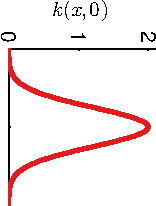
\includegraphics[width=\fwh,height=\fwb]{../figures/structure_examples/se_kernel}} 
& $\kernel_\textrm{SE}(\inputVar, \inputVar') = \sigma^2 \exp{\left(-\frac{(\inputVar - \inputVar')^2}{2\ell^2}\right)}$ \\
\rotatebox{90}{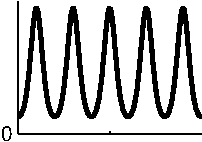
\includegraphics[width=\fwh,height=\fwb]{../figures/structure_examples/per_kernel}} 
& $\kernel_\textrm{Per}(\inputVar, \inputVar') = \sigma^2 \exp{\left(\frac{-2}{\ell^2}\sin^2(\frac{\pi|\inputVar - \inputVar'|}{p})\right)}$ \\
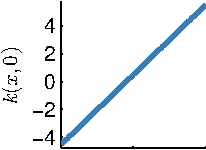
\includegraphics[width=\fwb,height=\fwh]{../figures/structure_examples/lin_kernel} 
& $\kernel_\textrm{Lin}(\inputVar, \inputVar') = \sigma_b^2 + \sigma_v^2(\inputVar - \ell)(\inputVar' - \ell)$
\end{tabular}
\caption{ Definitions of base kernels.  Left: a plot of each kernel as a function of one of its inputs.}
\label{fig:basic_kernels}
\end{figure}


Positive semidefinite kernels (\ie those which define valid covariance functions) are closed under addition and multiplication.
% \ie any algebraic composition of PSD kernels will define a PSD kernel.\fTBD{Cite theorem}
This allows one to create richly structured and interpretable kernels from well understood base components.
%Figure \ref{fig:kernels} shows several examples of structured kernels that can be constructed by adding or multiplying standard base kernels.
%
\newcommand{\fhbig}{1.8cm}
\newcommand{\fwbig}{2.4cm}
\newcommand{\kernpic}[1]{\includegraphics[height=\fhbig,width=\fwbig]{../figures/structure_examples/#1}}
\newcommand{\kernpicr}[1]{\rotatebox{90}{\includegraphics[height=\fwbig,width=\fhbig]{../figures/structure_examples/#1}}}
\newcommand{\largeplus}{\tabbox{{\Large+}}}
\newcommand{\largeeq}{\tabbox{{\Large=}}}
\newcommand{\largetimes}{\tabbox{{\Large$\times$}}}
\begin{figure}
\centering
\renewcommand{\tabularxcolumn}[1]{>{\arraybackslash}m{#1}}
%\begin{tabular}{m{\fwbig}m{0.01\textwidth}m{\fwbig}m{0.01\textwidth}m{\fwbig}m{\fwbig}m{\fwbig}}
\begin{tabular}{ccc}%{m{\fwbig}m{\fwbig}m{\fwbig}}
%\begin{tabularx}{\textwidth}{XXXXX|X|X}
%Composite & Draws from \gp{} & \gp{} posterior \\ \toprule
\kernpicr{se_times_per} & \kernpic{se_times_per_draws} & \kernpic{se_times_per_post} \\
SE $\times$ Per & \multicolumn{2}{c}{locally periodic} \\  \midrule
% \kernpicr{se_plus_per} & \kernpic{se_plus_per_draws} & \kernpic{se_plus_per_post} \\
% SE + Per & perdiodic with \newline local noise &  \\ \midrule
\kernpic{lin_times_lin} & \kernpic{lin_times_lin_draws} & \kernpic{lin_times_lin_post} \\
Lin $\times$ Lin  & \multicolumn{2}{c}{quadratic functions} \\ \midrule
% \kernpicr{se_times_lin} & \kernpic{se_times_lin_draws} & \kernpic{se_times_lin_post} \\
% Lin $\times$ SE  & increasing \newline local variation &  \\ \midrule
 \kernpic{lin_times_per} & \kernpic{lin_times_per_draws} & \kernpic{lin_times_per_post} \\
Lin $\times$ Per  & \multicolumn{2}{c}{growing amplitude}  \\ \midrule
 \kernpic{lin_plus_per} & \kernpic{lin_plus_per_draws} & \kernpic{lin_plus_per_post} \\
Lin + Per & \multicolumn{2}{c}{periodic with trend}  \\
\end{tabular}
\caption{ Examples of structures expressible by
  composite kernels.  
%The x-axis has the same scale for all plots.
  Left column: the composite kernel  Center: draws from a \gp{} with that kernel.  Right: \gp{} posterior after conditioning on three
  datapoints.
}
\label{fig:kernels}
\end{figure}


\paragraph{Summation}

Summation of kernels corresponds to the summation of independent functions in the following sense.
Suppose ${\function_1 \dist \GP(0, \kernel_1)}$, ${\function_2 \dist \GP(0, \kernel_2)}$ independently.
Then ${\function := \function_1 + \function_2 \dist \GP(0, \kernel_1 + \kernel_2)}$.
% \footnotemark.
%\footnotetext{
Additionally, the posterior of the component functions conditioned on observations of the sum are analytically tractable.
We make use of this in section \ref{sec:decomposing} to decompose learned kernels into interpretable components.

In one dimension, sums of kernels can express structure such as variation at multiple scales, or of the superposition of different function types.
For example, row 4 of figure~\ref{fig:kernels} shows the superposition of linear and periodic kernels/functions.

In multiple dimensions, summing kernels can correspond to decompositions of the form
\begin{equation}
\function(\inputVar_1, \inputVar_2) = \function_1(\inputVar_1) + \function_2(\inputVar_2)
\end{equation}
\ie `independent' variation in different dimensions.
%
\begin{figure}
\centering
\newcommand{\fha}{2.5cm}
\newcommand{\fwa}{3.4cm}
\newcommand{\addkernpic}[1]{{\includegraphics[height=\fha,width=\fwa]{../figures/additive_multi_d/#1}}}
\begin{tabular}{cc}
Kernel function & Draw from \gp{} \\
\toprule
\addkernpic{additive_kernel.pdf} & \addkernpic{additive_kernel_draw_sum.pdf} \\
$SE_1 + SE_2$ & $f_1(x_1) + f_2(x_2)$ \\
%$k_1(x_1,x_1') + k_2(x_2,x_2')$ & $f_1(x_1) + f_2(x_2)$  \\
%sum of 1D SE kernels & sum of 1D functions \\
%\midrule
\addkernpic{sqexp_kernel.pdf} & \addkernpic{sqexp_draw.pdf} \\
$SE_1 \times SE_2$ &  $f(x_1, x_2)$
%$k_1(x_1,x_1')k_2(x_2,x_2')$ & $f(x_1, x_2)$ \\
%product of & draw from\\
%1D SE kernels & product GP prior
\end{tabular}
\caption{A two-dimensional additive kernel, and a two-dimensional product kernel.  Left: a draw from an additive kernel corresponds to a sum of draws from one-dimensional kernels.  Right: functions drawn from a product kernel prior have less long-range dependency.
%In this example, both kernels are composed of one dimensional squared-exponential kernels, but this need not be the case in general.
}
\label{fig:multi_d_additivity}
\end{figure}

%
This is demonstrated in the first row of figure~\ref{fig:multi_d_additivity}.
%demonstrates a decomposition across dimensions.


\paragraph{Multiplication}

Multiplication of kernels does not correspond to a simple composition of functions; here, we give some examples of the properties that arise from multiplication of kernels.

%but allows for the construction of different structures and is best understood on a case by case basis\fTBD{Better language?}.
%
%For example, multiplying base kernels of the same form that act upon different dimensions of $\InputSpace$ can create the multidimensional generalisations of these kernels; this is true of \eg SE and LN\TBD{ reference a picture}.
%


Multiplying a kernel $\kernel$ by the SE kernel allows the structures implied by $\kernel$ to vary smoothly according the lengthscale of the SE kernel.  This is shown in row 2 of Figure \ref{fig:kernels}.
Multiplying a kernel by LN results in the amplitude of structures implied by $\kernel$ growing or shrinking linearly. This is shown in rows 4 and 5 of Figure \ref{fig:kernels}.
%\fTBD{Could perhaps perversely claim that multiplying by periodic results in wiggles being added to previous structure?}
%
%\fTBD{Can we do more than just give examples}

%In general, multiplying kernels can be thought of as an `AND' operation when viewing kernels as a measure of similarity.
%This arises since two points, $\inputVar,\inputVar'$, can only be considered similar by a product kernel function (\ie $\kernel_\textrm{prod}(\inputVar,\inputVar')$ is relatively large) if the points are considered similar by each component kernel function.

\paragraph{Interpretation}

To develop an intuition for the effect of combining two stationary kernels, we can note that the posterior mean function must be a weighted sum of kernel functions.  Thus, the third column of rows 1-2 of Figure \ref{fig:kernels} show the functions that can be combined linearly to produce the posterior means in the 5th column.

Loosely speaking, a sum of kernels can be understood as an `OR' operation: two points are considered similar if either kernel has a high value.
More precisely, we can express a sum of kernels as a concatenation of their features in the corresponding RKHS.

Complementarily, multiplying kernels can be loosely understood as an `AND' operation: two points are considered similar only if both kernels have a high value.
More precisely, we can express a product of kernels as a concatenation of the cartesian product of both kernels' features in the corresponding RKHS.

Combining multiple layers of AND and OR-like operators to construct complex functions is a common strategy.  For example, many vision models combine pooling and detection layers \TBD{cite}. In addition, AND/OR graphs \TBD{cite} and sum-product networks \TBD{cite} demonstrate the same compositional strategy.


\paragraph{Example expressions}

A number of standard model forms and interesting structures can be expressed as \gp s with composite kernels:

\begin{tabular}{l|l}
Bayesian linear regression & Lin \\
Bayesian quadratric regression & Lin $\times$ Lin \\
Bayesian polynomial regression & Lin $\times$ Lin $\times$ \dots\\
generalized Fourier decomposition & Per + Per + \dots \\
generalized additive models & $\sum_{d=1}^D \textrm{SE}_d$ \\
\gp{} with ARD kernel & $\prod_{d=1}^D \textrm{SE}_d$ \\
long-term trend & Lin + SE \\
growing amplitude & Lin $\times$ SE
\end{tabular}

In these expresssions, SE$_d$ denotes a squared-exponential kernel along the $d$th dimension.
We use the term 'generalized Fourier decomposition' to express the fact that the periodic functions capturable by a \gp{} with a periodic kernel are not limited to sine and cosines.


%\section{Gaussian Processes Priors}

%Gaussian processes are a flexible and tractable prior over functions, useful for solving regression and classification tasks\cite{rasmussen38gaussian}.
%The kind of structure which can be captured by a GP model is mainly determined by its \emph{kernel}: the covariance function.
%One of the main difficulties in specifying a Gaussian process model is in choosing a kernel which can represent the structure present in the data.
%For small to medium-sized datasets, the kernel has a large impact on modeling efficacy.
%\TBD{Note: The above paragraph is plagarized from my additive GP paper. -David} 

%
%The technique of constructing composite kernels using sums and products of existing kernels is not new \cite{rasmussen38gaussian} [more cites, Phil Hennig's astronomy work?].  
%However, the main contribution of this paper is to automate the search over kernel structures.

\section{Searching over structures}


As discussed above, we can construct a wide variety of kernel structures compositionally by adding and multiplying a small number of base kernels. In particular, we consider the four base kernel families discussed in Section \ref{sec:Structure}: squared exp (SE), periodic (Per), linear (Lin), and rational quadratic (RQ). Any algebraic expression combining these kernels using the operations $+$ and $\times$ defines a kernel family, whose hyperparaters are the concatenation of the hyperparameters for the base kernel families. 

Our search procedure begins by proposing all base kernels applied to all input dimensions. 

We allow the following search operators over our set of expressions:
\begin{itemize}
\item[(1)] Any subexpression $\subexpr$ can be replaced with $\subexpr + \baseker$, where $\baseker$ is any base kernel family.
\item[(2)] Any subexpression $\subexpr$ can be replaced with $\subexpr \times \baseker$, where $\baseker$ is any base kernel family.
\item[(3)] Any base kernel $\baseker$ may be replaced with any other base kernel $\baseker^\prime$.
\end{itemize}

We note that these operators can generate all possible algebraic expressions. To see this, observe that if we restricted the $+$ and $\times$ rules only to apply to base kernels, we would obtain a context-free grammar which generates the set of algebraic expressions. However, the more general versions of these rules allow more flexibility in the search procedure, since the CGF derivation may not be the most straightforward way to arrive at the kernel.

We search over this space using a greedy search: in each stage, we choose the $\numWinners$ highest scoring kernels and expand them by applying all possible operators.

Our search operators are motivated by strategies researchers often use in constructing kernels. In particular,
\begin{itemize}
\item We look for structure such as periodicity in the residuals of a model, and then extend the model to capture that structure. This corresponds to applying rule (1).
\item We start with structure (such as periodicity) which is supposed to hold globally, but find that it only holds locally. This corresponds to applying rule (2) to obtain the structure shown in row 1 of Figure \ref{fig:kernels}.
\item We add features incrementally using algorithms like boosting, backfitting, or forward selection. These correspond to applying rules (1) or (2) to new dimensions not yet included in the model.
\end{itemize}

\paragraph{Scoring kernel families}

Choosing kernel structures requires a criterion for evaluating the structures. We choose marginal likelihood as our criterion, because it tests both interpolation and extrapolation and because it directly penalizes the complexity of the prior over functions \cite{rasmussen2001occam}.  In a fully Bayesian approach, we would put priors over the hyperparameters and compute the marginal likelihood of the models with all the hyperparameters integrated out. However, as this would be difficult to do across our space of models, we approximate this integral by choosing the parameters to optimize the marginal likelihood, and then apply the Bayesian information criterion (BIC) to penalize model complexity. \TBD{If true, say we got similar results using Laplace} We note that other model selection criteria could be used with our search procedure. For instance, random cross-validation could be used when the goal is interpolation.

Unfortunately, optimizing over hyperparameters is not a convex optimization problem, and the space can have many local optima. For instance, for the example in Figure \ref{fig:mauna_grow} can be modeled with a short length scale and small noise or a long length scale and large noise, and both explanations are better than any intermediate ones. Similarly, in data with periodic structure, integer multiples of the true period are often local optima. 

To deal with this, we take advantage of our greedy search procedure in order to get smart initializations: all of the hyperparameters which were part of the previous model are initialized to their previous values. The hyperparameters are then optimized using conjugate gradients, randomly restarting the newly introduced hyperparameters. While this procedure isn't guaranteed to find the global optimum, we offer some heuristic motivations:
\begin{itemize}
\item We (as researchers) often choose kernel structures by looking at the residuals and coming up with a model for those. This is analogous to applying rule (1), adding a new kernel but keeping the old hyperparameters fixed.
\item If a simple structure includes a periodic kernel, the learned period is likely to be approximately correct even if the true structure turns out to be more complex.
\end{itemize}





%The discussion above demonstrates that rich structure can be captured with summation and multiplication of simple base kernels.
%We therefore consider searching over all kernel structures that can be expressed as sums and products of base kernels. \TBD{RBG: need (1) 1-2 sentences about what a CFG is, what production rules are; (2) an example derivation, e.g. for Mauna; (3) say that production rules are supposed to correspond to motifs of probabilistic modeling}

%\begin{center}
%\begin{tabular}{rccc}
%\textrm{Replacement} & $\kernel_i$ & $\to$ & $\kernel'_i$\\% & $\forall\, \kernel' $\\
%\textrm{Addition} & $\kernel_i$ & $\to$ & $\kernel_i + \kernel'_j$\\% & $\forall\, j,\kernel' $\\
%\textrm{Multiplication} & $\kernel_i$ &  $\to$ & $\kernel_i \times \kernel'_j$\\% & $\forall\, j,\kernel'$\\
%\end{tabular}
%\end{center}

%Details of the search algorithm are given in the supplementary material \TBD{For now}.

%\paragraph{A greedy search algorithm}
%Our search starts by first proposing all base kernels applied to all input dimensions.  We then choose the kernel with the highest approximate marginal likelihood, apply all expansions to this kernel, and repeat this process for a fixed number of steps.

%We optimized kernel hyperparameters at each step using conjugate gradients, randomly restarting any newly introduced kernel hyperparameters.  To approximate the marginal likelihood of a kernel without integrating over hyperparameters, used the Bayesian Information Criterion (BIC)\footnotemark \TBD{cite}.
%We also experimented with using the Laplace approximation to the marginal likelihood, but this was found to be less numerically stable and was not meaningful in cases when the optimiser failed to reach an optimum.
%\footnotetext{Because BIC is a function of the number of parameters in a model, we adjusted for cases where two parameters were only serving the role of one.  \eg when two kernels are multiplied, one of the variance parameters becomes redundant.}




\section{Related Work}
\label{sec:related_work}

\paragraph{Composite kernels in GP models} The technique of constructing composite kernels using sums and products of existing kernels was demonstrated in detail in Chapter 5 of \cite{rasmussen38gaussian}, where the resulting posterior mean was also decomposed into a sum of component-wise means, although the posterior variance was not.  Our work can be viewed as an extension and automation of this approach.

\paragraph{Generalized Additive Models} \cite{hastie1990generalized} are models in which the posterior mean can be expressed $\expect[f(\vx)] = \sum_{d=1}^D f_d(x_d)$. These models have a limited compositional form, but one which is interpretable.  We compare against this model in our multi-dimensional experiments.

\cite{plate1999accuracy} constructs a \gp{} with a composite kernel, summing an SE kernel along each dimension, with an SE-ARD kernel on all dimensions.  This model is motivated by the desire to specify the trade off between the interpretability of additive models and the flexibility of multiplicative models.

\paragraph{Compositional model search for unsupervised learning} \cite{grosse2012exploiting} performed a greedy search over a compositional model class for unsupervised learning.  Their models were composed of sums and element-wise products of random variables defined on matrices.  This model class contained a large number of existing unsupervised models as special cases.  Earlier work in unsupervised Bayseian structure discovery was done in \cite{kemp2008discovery}.

\paragraph{ANOVA Kernels}

Support vector regression with ANOVA decomposition kernels \cite{stitson1999support}

%\subsubsection{Smoothing spline ANOVA models}
A closely related procedure from the statistics literature is smoothing-splines ANOVA (SS-ANOVA)\cite{wahba1990spline, gu2002smoothing}.
This model is a weighted sum of splines along each dimension, plus a sum of splines over all pairs of dimensions, all triplets, etc, with each individual interaction term having a separate weighting parameter.
Learning in SS-ANOVA is usually done via penalized-maximum likelihood with a fixed sparsity hyperparameter.
Because the number of terms to consider grows exponentially in the order, in practice, only terms of first and second order are usually considered.  This model is similar to ours, if we were to restict our attention to spline kernels

\paragraph{Additive Gaussian Processes} \cite{duvenaud2011additive11} is a Gaussian process model whose kernel implicitly sums over all $2^D$ possible products of one-dimensional base kernels.  
However, this model's parameterization is not as flexible as the kernels expressible in our grammar.

\paragraph{Hierarchical Kernel Learning}

%In "High-Dimensional Non-Linear Variable Selection through Hierarchical Kernel Learning", Bach
\cite{DBLP:journals/corr/abs-0909-0844} uses a regularized optimization framework to learn a weighted sum over an exponential number of kernels which can be computed in polynomial time.
The subsets of kernels considered by this method are restricted to be a \textit{hull} of kernels. In the setting we are considering in this paper, a hull can be defined as a subset of all terms such that if term $\prod_{j \in J} k_j(\bf x, x')$ is included in the subset, then so are all terms $\prod_{j \in J / i} k_j(\bf x, x')$, for all $i \in J$.
%For details, see \cite{DBLP:journals/corr/abs-0909-0844}.
%Given each dimension's kernel, and a pre-defined weighting over all terms, HKL performs model selection by searching over hulls of interaction terms.
% \subsubsection{All-subsets kernel with uniform weightings}
%In \cite{DBLP:journals/corr/abs-0909-0844}, Bach also fixes the relative weighting between orders of interaction with a single term $\alpha$, computing the sum over all orders by:
%\begin{equation}
%\label{eqn:uniform}
%k_{a}({\bf x, x'}) = v_D^2 \prod_{d=1}^D \left(1 + \alpha k_{d}(x_{d}, x_{d}') \right)
%\end{equation}
%which has computational complexity $O(D)$.
%However, this formulation forces the weight of all $n$th order terms to be weighted by $\alpha^n$.
%
The main difficulty with this approach is that hyperparameters are hard to set other than by cross-validation. 
%In contrast, our method optimizes the hyperparameters of each dimension's base kernel, as well as the relative weighting of each order of interaction. 



%A related functional ANOVA GP model\cite{kaufman2010bayesian} decomposes the \emph{mean} function into a weighted sum of GPs.
%However, the effect of a particular degree of interaction cannot be quantified by that approach.
%Also, computationally, the Gibbs sampling approach used in \cite{kaufman2010bayesian} is disadvantageous.

\paragraph{Genetic Searches over Kernel Structures}
A similar method was developed by \cite{diosan2007evolving} using SVMs in place of Gaussian processes, cross-validation error instead of marginal likelihood, and a genetic algorithm instead of a greedy search.  
In \cite{bing2010gp}, a genetic programming construction and optimization method was used to select a kernel for relevance vector machines.

\paragraph{Equation Learning}
A related body of work with similar goals are the various approaches to equation learning.  
For example, \cite{schmidt2009distilling}, \cite{todorovski1997declarative} and \cite{washio1999discovering} attempt to learn parametric forms of equations to describe time series, or relations between quantities.  The advantage of a \gp{}-based approach is that non-parametric structure can be represented even within an interpretable decomposition.  For example, while equation-learning methods could recover a function with a sine-wave component composed with other structure, our procedure can represent \emph{any} periodic function composed with other structure.

\paragraph{Semiparametric Regression}
Semiparametric regression \TBD{add cites} attempts to combine interpretability with flexibility by building  a composite model out of an interpretable, parametric part (such as linear regression) and a ``catch-all'' nonparametric part (such as a \gp{} with an SE kernel).
Structure search has the same goal, but improves upon semiparametric regression in two ways.
First, construcing a compound model through structure in the kernel allows us to integrate over the parameters of the implicit components of the model.
Second, by automatically searching over components, we remove the limitation that the practictioner must be able to specify in advance the parametric form of any part of the model.


\paragraph{Multiple Kernel Learning}
There is a large body of work attempting to construct a rich kernel through a weighted sum of base kernels, including in \gp{} models.  
\cite{christoudias2009bayesian}
\TBD{cite more} 
However, these methods typically construct all kernels in advance, and simply reweight them.  This sort of approach would be inapplicable in our case, since our search space is exponential in our search depth, and we also must estimate the hyperparameters of each kernel.%One could imagine expanding our search for some fixed depth, instantiating a sum of all
%In the \gp{} framework,  showed how mixtures of kernels can be learnt by gradient descent in the Gaussian process framework.
%They call this \emph{Bayesian localized multiple kernel learning}.

\paragraph{Nonparametric kernel functions}

Since the complexity of our kernel is bounded only by the search depth, we could consider the structure search to be a non-parametric kernel model - in a sense, a doubly nonparametric model.  However, there has been some similar work along these lines in \cite{salakhutdinov2008using}, where a deep neural network was use to learn the kernel of a \gp{}.

%Hyperkernels \cite{ong2002hyperkernels}

\section{Validation on synthetic data}

We validate our method by constructing synthetic data sets to check that we can infer known structure.
For several composite kernel expression we construct synthetic data by uniformly sampling 300 input points in a symmetric hyper cube of and then sample a Gaussian process over these data points.
We then add \iid Gaussian noise to the output data with variance chosen to achieve a particular signal to noise ratio (SNR\footnotemark).
\footnotetext{We define the signal to noise ratio to be the standard deviation of the function divided by the standard deviation of the noise.}

Table~\ref{tbl:synthetic} lists the composite kernels we used to generate data (underscores indicate which dimension each kernel applied to) and the diemsionality, $d$, of the input space, together with those inferred by our search.
When SNR is highest, the model correctly infers the structure of the kernel; in fact it also discovers unintentionally introduced linear structure\footnotemark!\fTBD{Currently re-running experiments with shorter lengthscales to check we are not kidding ourselves}.
\TBD{Comment about higher noise regimes when data in.}

\footnotetext{Random samples from SE kernels with long length scales occasionally resulted in near linear trends in the data which were only noticed after running the search algorithm.}

\begin{table*}[ht!]
\caption{{\small
Kernels used to generate synthetic data together, dimensionality, $d$, of the input space and the inferred kernels at different signal to noise ratios (SNR).
}}
\label{tbl:synthetic}
\begin{center}
\begin{tabular}{c c | c c c}
Kernel & $d$ & SNR = 10 & SNR = 2 & SNR = 1 \\
\hline
$\SE + \RQ$                               & 1 & \ldots \\
$\Lin \times \Per$                        & 1 & $\Lin \times \Per$ \\
$\SE_1 + \RQ_2$                           & 2 & $\SE_1 + \RQ_2$ \\
$\SE_1 + \SE_2 \times \Per_1 + \SE_3$     & 3 & $\SE_1 + \SE_2 \times \Per_1 + \SE_3 \times \Lin_2$ \\
$\SE_1 \times \SE_2$                      & 4 & $\SE_1 \times \SE_2 \times \Lin_1$ \\
$\SE_1 \times \SE_2 + \SE_2 \times \SE_3$ & 4 & \ldots\\
$(\SE_1 + \SE_2) \times (\SE_3 + \SE_4)$  & 4 & $(\SE_1 + \SE_2) \times (\SE_3 + \SE_4\times\Lin_4)$\\
\end{tabular}
\end{center}
\end{table*}

\section{Structure discovery in time series}

%In this section, we show on several time series datasets both the kernel expression found by our search, and the complete \gp{} posterior distribution implied by that kernel and the data.  
%We then also plot that same kernel and posterior decomposed into additive components.

We ran our method on several time series datasets in order to test whether it learns plausible and interpretable structure. 
For these datasets, we show both the best kernel expressions found in each stage of the search, and the complete posterior distribution implied by that kernel and the data. 
Additionally, we show decompositions of the time series into superpositions of components as implied by the kernel structure.
We pay special attention to the models' extrapolations beyond the range of observed data, since this is a strong test of the correctness of the learned structure.

In these experiments, the search was run up to depth 10, and all of the base kernels from Section \ref{sec:Structure} were used.

%\section{Decomposing a function}

%Sums of kernels were shown in section~\ref{sec:Structure} to correspond to sums of independent functions.
%By splitting kernel expressions found by our search algorithm into additive components, we can also decompose the \gp{} posterior over functions into a joint distribution over functions that are summed togther.
%This potentially allows us to probabilistically separate causally the independent processes that give rise to the data. 

%\TBD{RBG: It's not immediately obvious that this section is part of the experiments. Also, maybe consider moving it till after the quantitative comparisons?  It could be useful rhetorically to first ask, ``how well does our algorithm do,'' and then ``let's find out why it works.''}

\paragraph{Decomposing a sum kernel}
\label{sec:decomposing}
%We can analytically decompose a \gp{} posterior distribution over additive components using the following identity:
Given a composite kernel consisting of a sum of several simpler kernels, we can analytically infer a decomposition of a function into a sum of the components.
For simplicity, consider the case of a sum of two kernels.
Let $\function = \function_1 + \function_2$, where $\function_1 \sim \GP( \vmu_1, k_1)$ and $\function_2 \sim \GP( \vmu_2, k_2)$.
The conditional distribution of the component $\function_1$ conditioned on $\function$ is given by:
\begin{align}
\function_1 | \function \sim \mathcal{N} \Big( & \vmu_1 + \vk_1\tra (\vK_1 + \vK_2)\inv \left( \function - \vmu_1 - \vmu_2 \right), \nonumber \\
& \vk_1 - \vk_1\tra (\vK_1 + \vK_2)\inv \vk_1 \Big).
\end{align}
\TBD{RBG: In the variance formula, we're subtracting a vector and a scalar. Should the first term be the constant $k_1(x, x)$?
Also, I was confused by the notation; I originally read this as a distribution over a function, whereas really it's a distribution over the value of the function at some point $x$.
Can we change the notation to make this explicit?}
%and the covariance between the two components, conditioned on their sum is given by:
%\begin{align}
%\cov(\vf_1^\star, \vf_2^\star) | \vf = \vk_1^{\star\tra} (\vK_1 + \vK_2)\inv \vk_2^\star
%\end{align}
%Derivations can be found in the supplementary material.

%In cases where the kernel expression contains any product of a sum, our software automatically expands out the expression into an equivalent sum of products.  This operation transforms the posterior into a more interpretable, but equivalent, form.
All of the kernels in our search space can be written as sums of products of base kernels by applying the distributive rule. This often leads to interpretable decompositions, even when the learned kernel was not originally of this form.



\label{sec:extrapolation}
\paragraph{Mauna Loa Atmospheric Carbon Dioxide}

First, we revisited a dataset explored in \cite{rasmussen38gaussian}, pages 120-126, where a kernel was hand-tailored to fit a \gp{} model to the dataset.

%Figure \ref{fig:mauna_grow} show the posterior of the increasingly appropriate model as the search depth increases on this dataset.
%Note in particular that, while the data can be smoothly interpolated by a single base kernel model, the extrapolations improve dramatically as the search depth increases.

Figure \ref{fig:mauna_decomp} shows the complete posterior of the model chosen by our method, together with the posteriors of the additive components.
The plot shows a plausible extrapolation and interpretable components: a long-term trend, annual periodicity, medium-term deviations and short-term serially correlated `noise'.  We also plot the residuals, in order to indicate that there is little obvious structure left in the data.

\begin{figure*}[h!]
\centering
\newcommand{\wmg}{5.5cm}  % width maunu growth
\newcommand{\hmg}{4cm}  % height maunu growth
\begin{tabular}{c}
 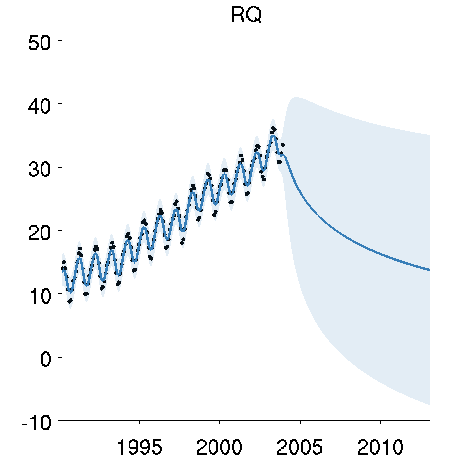
\includegraphics[width=\wmg,height=\hmg]{../figures/decomposition/03-mauna2003-s_max_level_0/03-mauna2003-s_all_small} 
 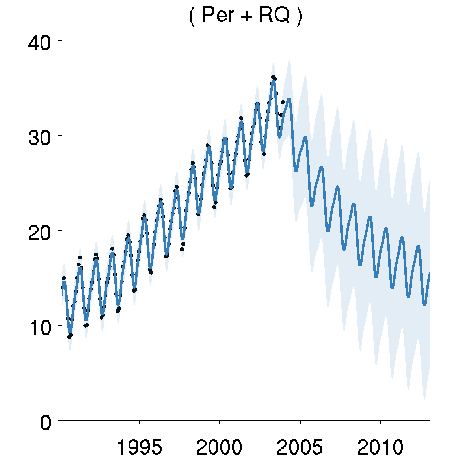
\includegraphics[width=\wmg,height=\hmg]{../figures/decomposition/03-mauna2003-s_max_level_1/03-mauna2003-s_all_small}
 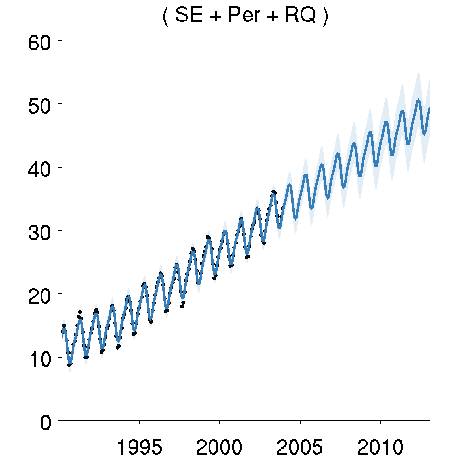
\includegraphics[width=\wmg,height=\hmg]{../figures/decomposition/03-mauna2003-s_max_level_2/03-mauna2003-s_all_small}
\end{tabular}
\caption{Posterior mean and variance for different depths of kernel search.  In the first row, the function is only modeled as a locally smooth function, and the extrapolation is extemely poor.  In the second, a periodic component is added, and the extrapolation is better.  At depth 3, the kernel can capture most of the relevant structure, and is able to extrapolate reasonably. %\TBD{RBG: (1) I think we somehow need to visualize the lengthscales, to make it obvious that the SE kernels really mean different things. (2) Why isn't SE + PE the correct answer?}
}
\label{fig:mauna_grow}
\end{figure*}

\begin{figure}[h!]
\newcommand{\wmgd}{9.5cm}  % width mauna decomp
\newcommand{\hmgd}{3.1cm}  % height mauna decomp
\newcommand{\mdrd}{../figures/decomposition/11-Feb-03-mauna2003-s}  % mauna decomp results dir
\begin{tabular}{c}
\hspace{-1cm} 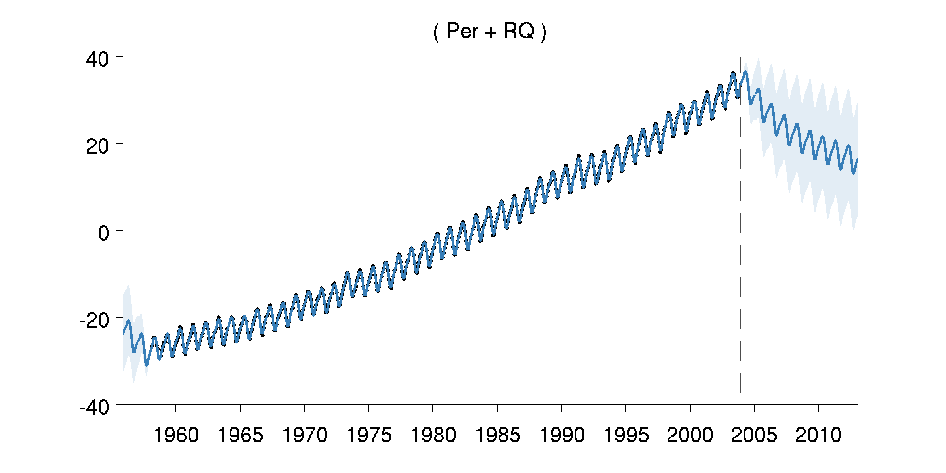
\includegraphics[width=\wmgd,height=\hmgd]{\mdrd/03-mauna2003-s_all} \\ = \\
\hspace{-1cm} 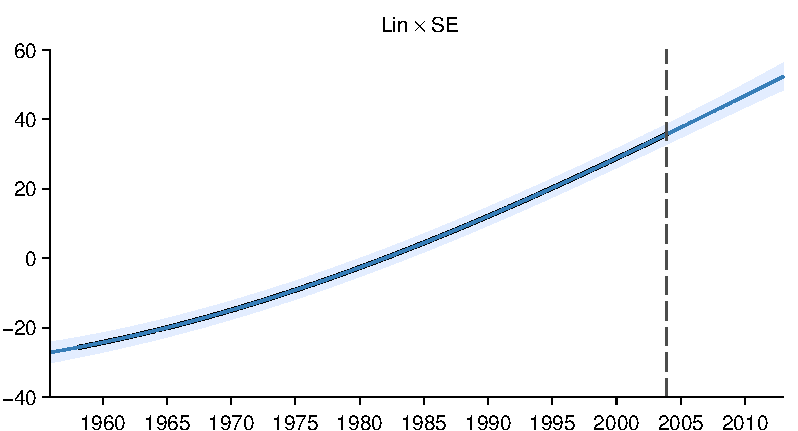
\includegraphics[width=\wmgd,height=\hmgd]{\mdrd/03-mauna2003-s_1} \\ + \\
\hspace{-1cm} 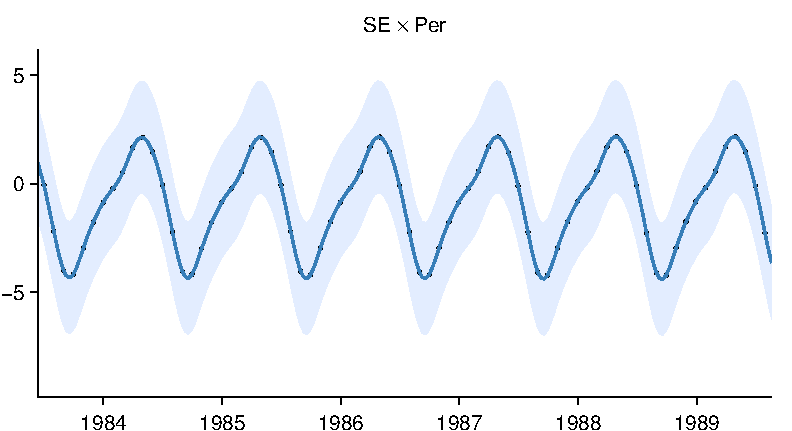
\includegraphics[width=\wmgd,height=\hmgd]{\mdrd/03-mauna2003-s_2_zoom} \\ + \\
\hspace{-1cm} 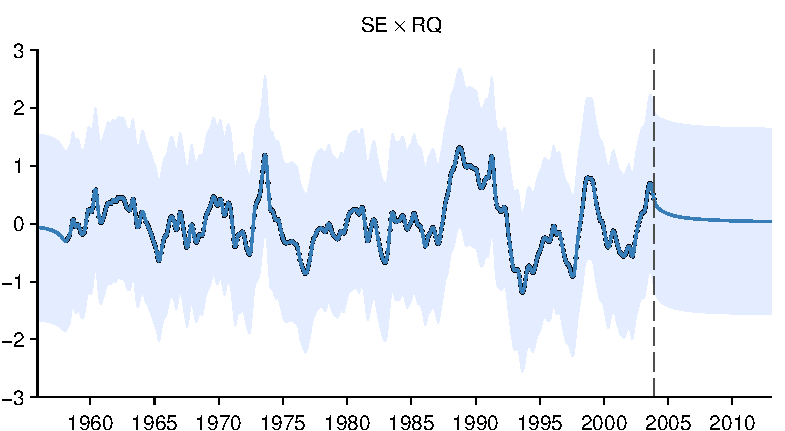
\includegraphics[width=\wmgd,height=\hmgd]{\mdrd/03-mauna2003-s_3} \\ + \\
\hspace{-1cm} 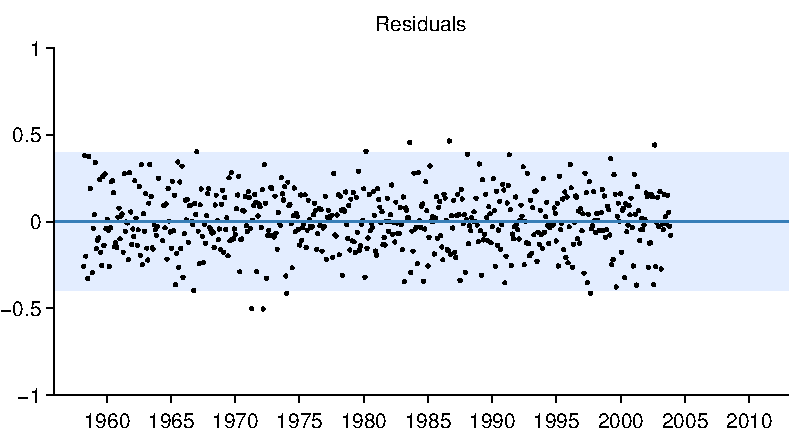
\includegraphics[width=\wmgd,height=\hmgd]{\mdrd/03-mauna2003-s_resid}
\end{tabular}
\caption{First row: The posterior on the Mauna Loa dataset after a search of depth 8.  Subsequent rows: automatic decomposition of Mauna Loa data.  The signal has been automatically decomposed into long-term, yearly periodic, medium-term anomaly and short-term noise components, respectively. Note that in the third row, the scale has been changed in order to clearly show the yearly periodic structure.}
\end{figure}
\label{fig:mauna_decomp}

\paragraph{Airline passenger data}

\TBD{Give an intro to this dataset.}
Figures \ref{fig:airline_grow} and \ref{fig:airline_decomp} show the corresponding plots for the airline data set (\TBD{describe me!}).
\TBD{Make similar observations of good performance}

Note that the linear kernel allows an element of heteroskedasticity in our model - the posterior marginal variance grows with the increase in the number of passengers over time.

\begin{figure}[h!]
\centering
\newcommand{\wag}{4.8cm}  % width airline growth
\newcommand{\hag}{4cm}  % height airline growth
\begin{tabular}{cc}
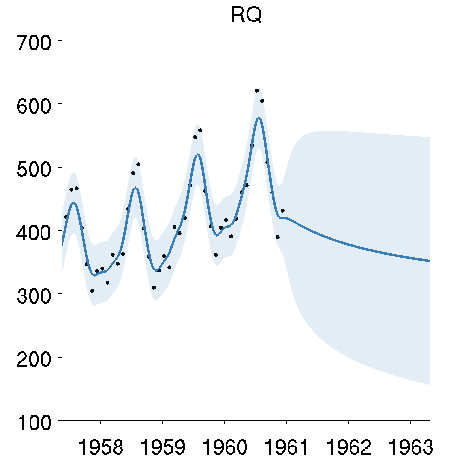
\includegraphics[width=\wag,height=\hag]{../figures/decomposition/01-airline-s_max_level_0/01-airline-s_all_small}
\hspace{-1cm} 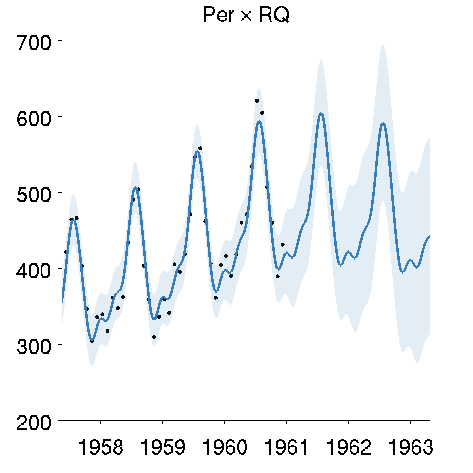
\includegraphics[width=\wag,height=\hag]{../figures/decomposition/01-airline-s_max_level_1/01-airline-s_all_small} \\
\hspace{-1cm} 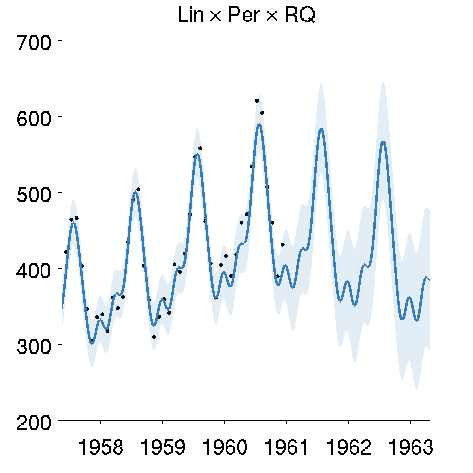
\includegraphics[width=\wag,height=\hag]{../figures/decomposition/01-airline-s_max_level_2/01-airline-s_all_small} 
\hspace{-1cm} 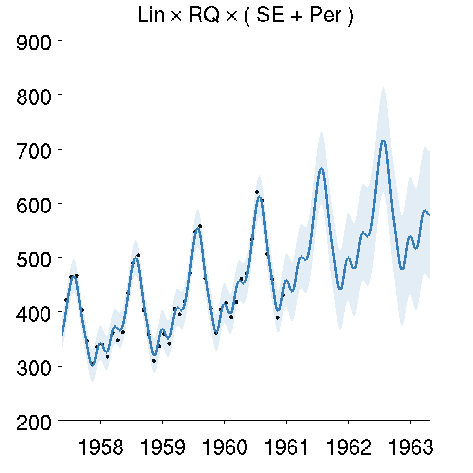
\includegraphics[width=\wag,height=\hag]{../figures/decomposition/01-airline-s_max_level_3/01-airline-s_all_small}
\end{tabular}
\caption{Posterior mean and variance for different levels of kernel search on the airline dataset. \TBD{RBG: it looks like the figures on the left got clipped.}}
\label{fig:airline_grow}
\end{figure}

% Created by the command:
% postprocessing.make_all_1d_figures(folder='../results/31-Jan-1d/', prefix='31-Jan-v3', rescale=False)

\begin{figure}[h!]
\centering
\newcommand{\wagd}{9.5cm}  % width airline decomp
\newcommand{\hagd}{3.5cm}  % height airline decomp
%\newcommand{\ard}{../figures/decomposition/11-Feb-01-airline-s}  % airline results dir
\newcommand{\ard}{../figures/decomposition/31-Jan-v301-airline-months}  % airline results dir
\begin{tabular}{c}
\hspace{-1cm}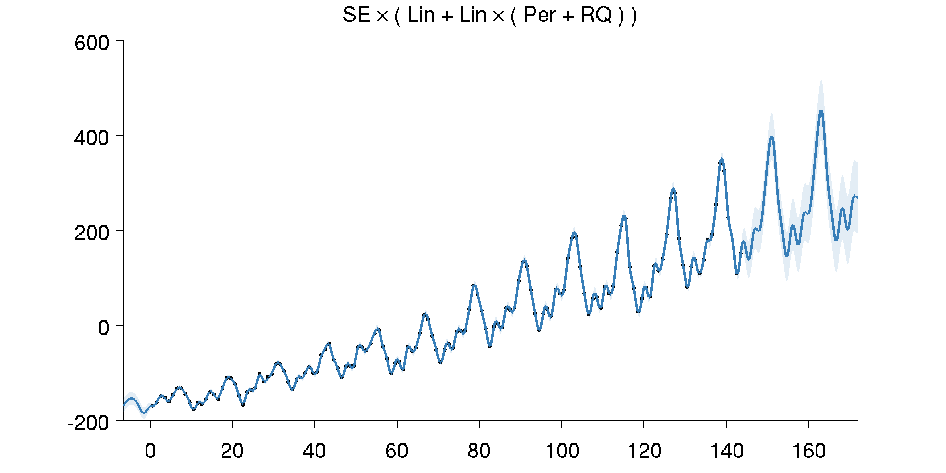
\includegraphics[width=\wagd,height=\hagd]{\ard/01-airline-months_all} \\
 = \\ 
%\hspace{-1cm} 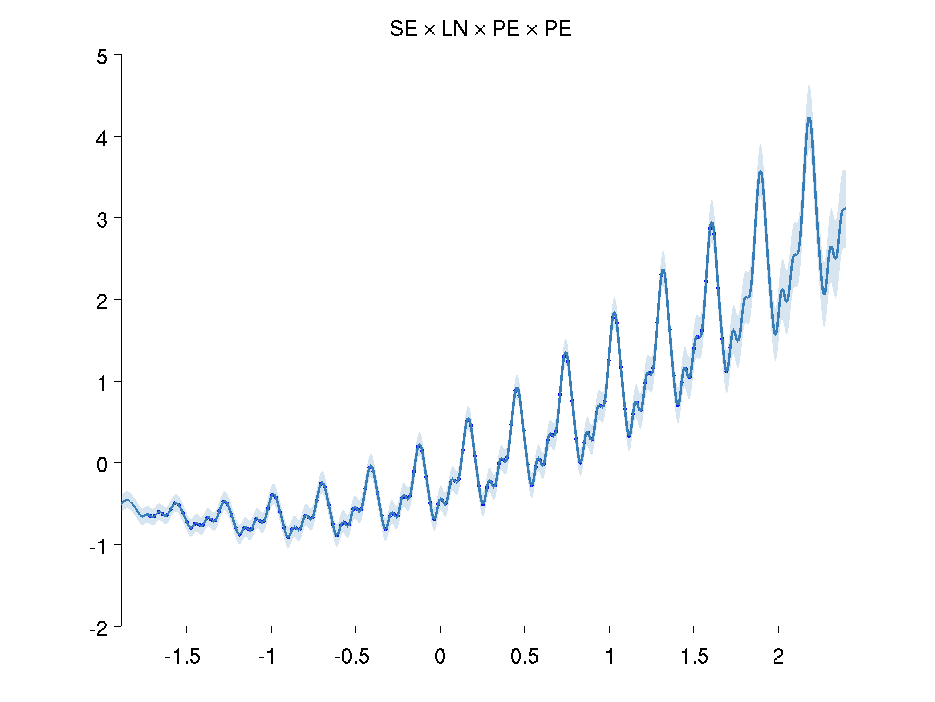
\includegraphics[width=\wagd,height=\hagd]{\ard/01-airline-s_4} \\
% + \\
\hspace{-1cm} 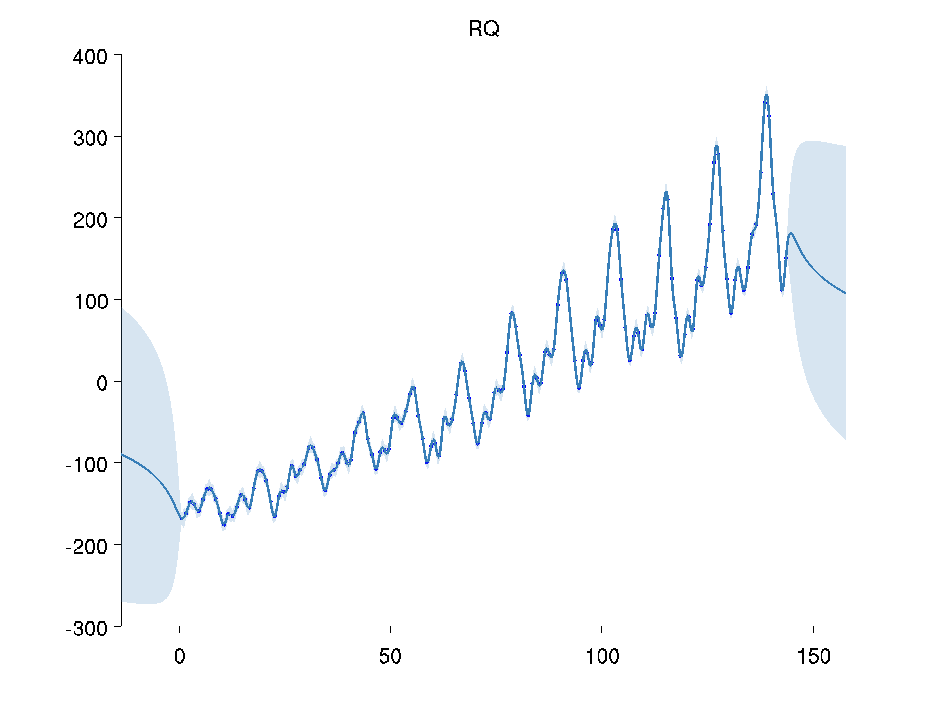
\includegraphics[width=\wagd,height=\hagd]{\ard/01-airline-months_1} \\
 + \\
\hspace{-1cm}  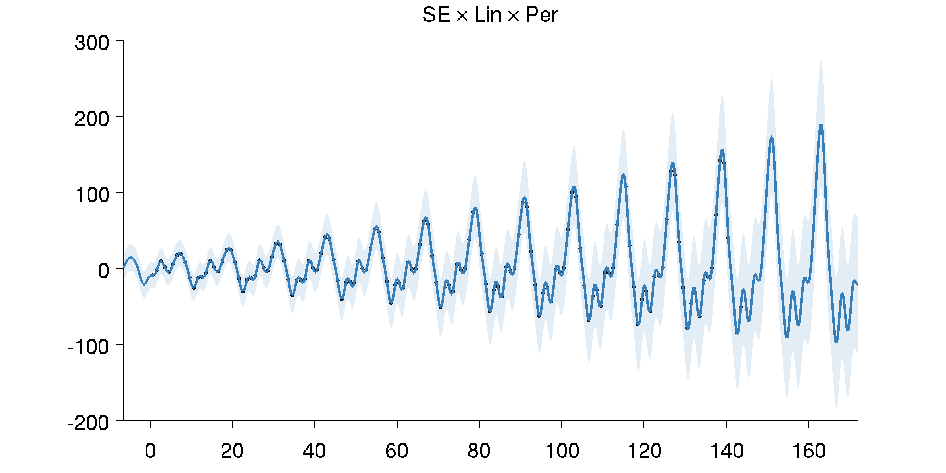
\includegraphics[width=\wagd,height=\hagd]{\ard/01-airline-months_2} \\
 + \\
\hspace{-1cm}   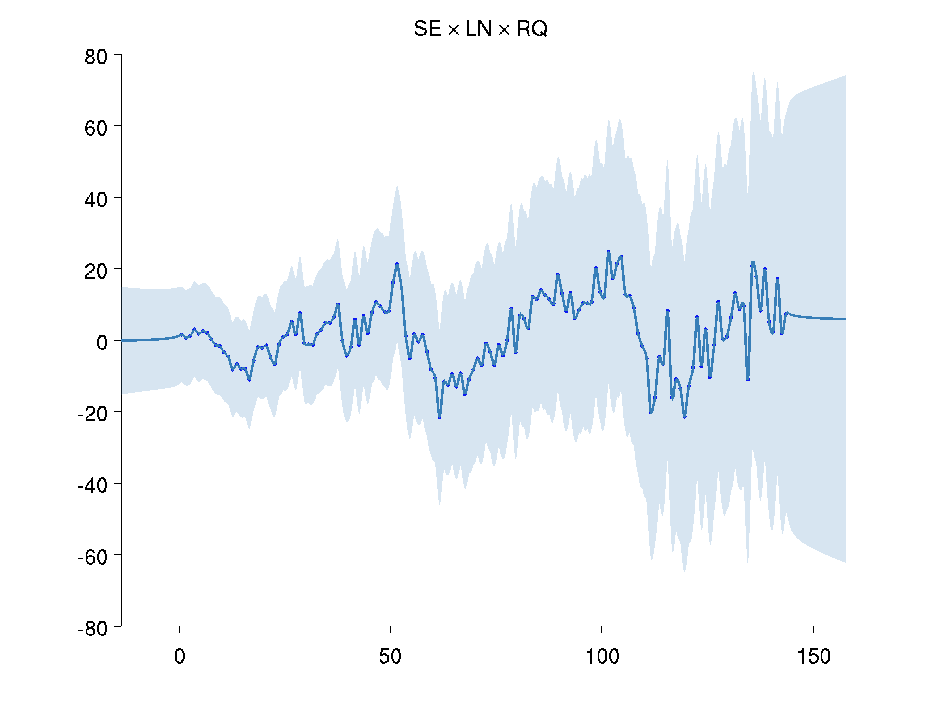
\includegraphics[width=\wagd,height=\hagd]{\ard/01-airline-months_3} \\
 + \\
\hspace{-1cm} 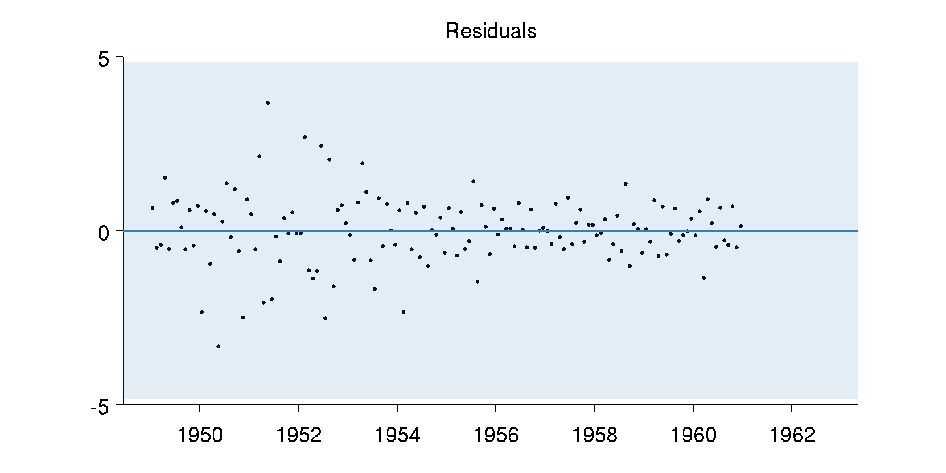
\includegraphics[width=\wagd,height=\hagd]{\ard/01-airline-months_resid}
\end{tabular}
\caption{First row:  The airline dataset and posterior after a search of depth 8.  Rows 2-4: Additive decomposition of posterior into long-term smooth trend, yearly variation, and short-term noise.  Note that the variance of the noise grows over time, making this a heteroskedastic model. 
%\TBD{RBG: We allow heteroskedastic noise in our models?}
}
\label{fig:airline_decomp}
\end{figure}

%To evaluate the effectiveness of our method we performed two types of experiments.
%First, we examined the ability of our algorithm to discover useful structure in one-dimensional datasets.  Second, we examined the predictive performance of our model on multi-dimensional datasets.
% testing the ability of the algorithm to infer both an accurate regression function estimate and to produce an interpretable decomposition of a regression function.
%The accuracy experiments show that our method consistently matches or beats previous state of the art regression methods (\TBD{not yet statistically significantly within each experiment - more experiments currently running\ldots}).
%The decomposition experiments produce highly interpretable decompositions of time series data and highly plausible extrapolations; a particularly rare property of naively applied (linear) smoothers (\TBD{justify comment - e.g.~local linear is just linear, GP Sq-Exp nose dives towards the mean}).

\paragraph{Solar Irradiance Data} 
We next analyzed a time series of annual solar irradiation data from 1610 to 2011 \cite{lean1995reconstruction}.
%
\begin{figure}[h!]
\newcommand{\wsd}{9.5cm}  % width solar decomp
\newcommand{\hsd}{4cm}  % height solar decomp
\newcommand{\srd}{../figures/decomposition/11-Feb-02-solar-s}  % solar decomp results dir
\begin{tabular}{c}
\hspace{-1cm} 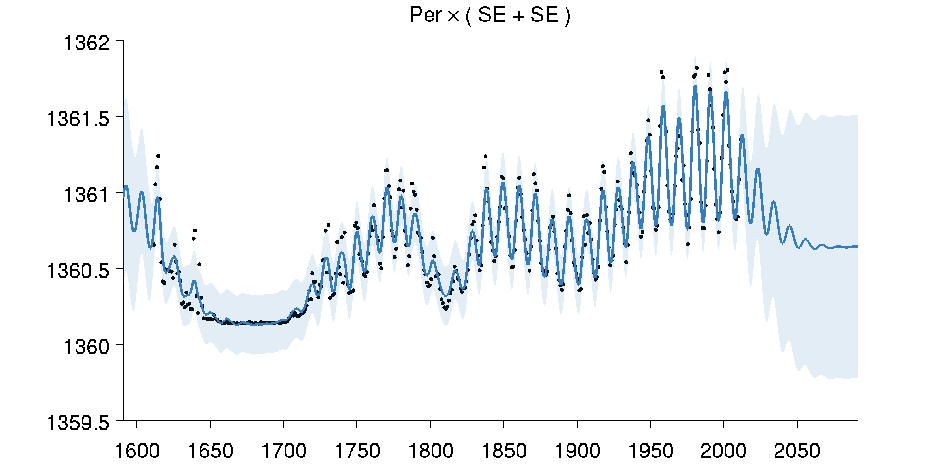
\includegraphics[width=\wsd,height=\hsd]{\srd/02-solar-s_all} \\
%\\ = \\
%\hspace{-1cm} 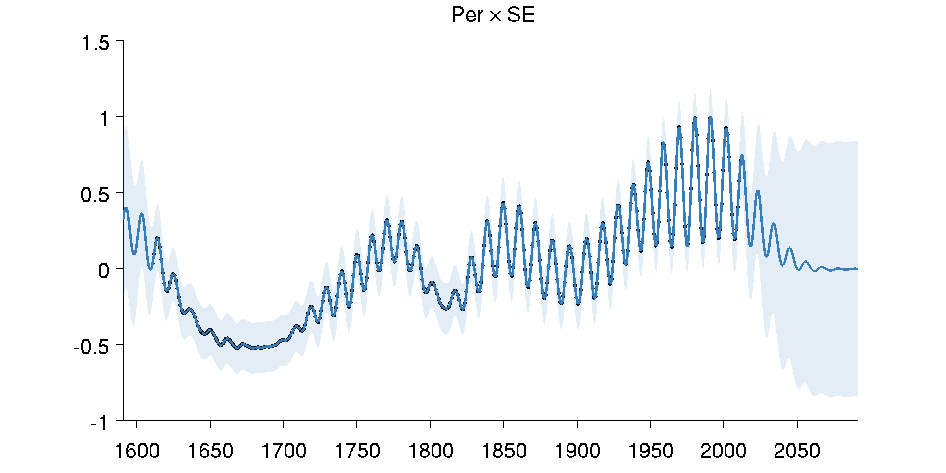
\includegraphics[width=\wsd,height=\hsd]{\srd/02-solar-s_1} \\ + \\
%\hspace{-1cm} 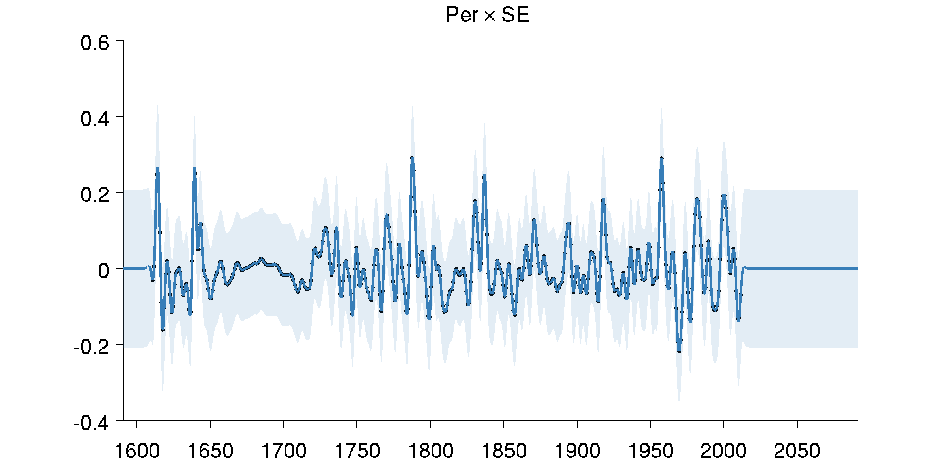
\includegraphics[width=\wsd,height=\hsd]{\srd/02-solar-s_2} \\ + \\
\hspace{-1cm} 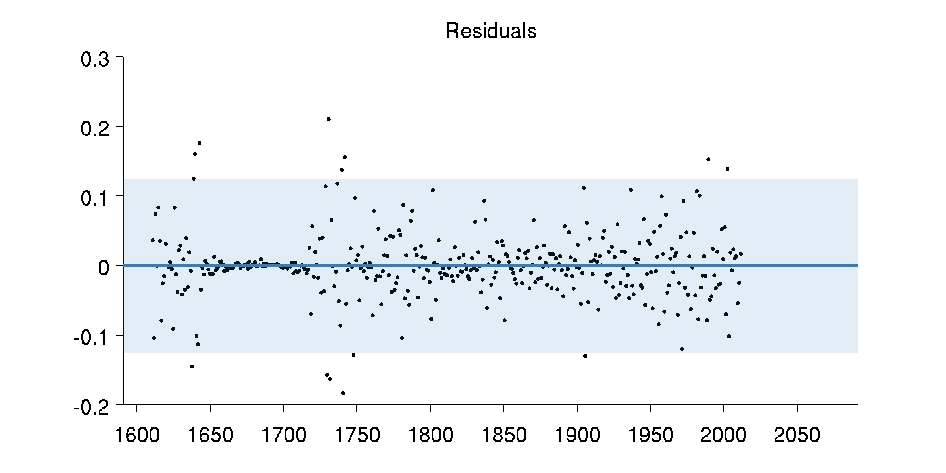
\includegraphics[width=\wsd,height=\hsd]{\srd/02-solar-s_resid}
\end{tabular}
\caption{Full posterior and residuals on the solar irradiance dataset.}
\label{fig:solar_decomp}
\end{figure}
%
Figure \ref{fig:solar_decomp} shows the posterior and residuals of the learned kernel on this dataset.
While our model captures the periodic trend in the data, it misses out on another aspect of the data: the flat period from 1645 to 1715 which contains no periodicity and has much smaller variance than the rest of the dataset.
This corresponds to the Maunder minimum, a period in which sunspots were extremely rare.
None of the models in our search space are capable of representing this structure, since all of the base kernels apart from Lin are stationary, and it is hard to see how Lin would help in modeling this structure.
Despite the inability to model the Maunder minimum, our approach fails gracefully: the learned kernel still captures the overall periodic structure and longer term trends, and makes plausible extrapolations.
It is likely that our framework could be extended to capture nonstationary structure by adding a changepoint kernel \TBD{cite?}.

\paragraph{Multidimensional decomposition}  Decomposition of multi-dimensional posteriors into sums of one-dimensional functions is possible as well, and was demonstrated in \cite{duvenaud2011additive11}.  \fTBD{Probably citing myself too much...}

\section{Quantitative evaluation}

%In addition to producing highly interpretable decompositions of regression functions, our method also produces state of the art predictions in both extrapolation and interpolation tasks.
In addition to the qualitative evaluation in the previous section, we also investigated quantitatively how our method performs on both extrapolation and interpolation tasks.

\subsection{Extrapolation}

\begin{figure}[h!]
\centering
\begin{tabular}{c}
\hspace{-0.5cm} 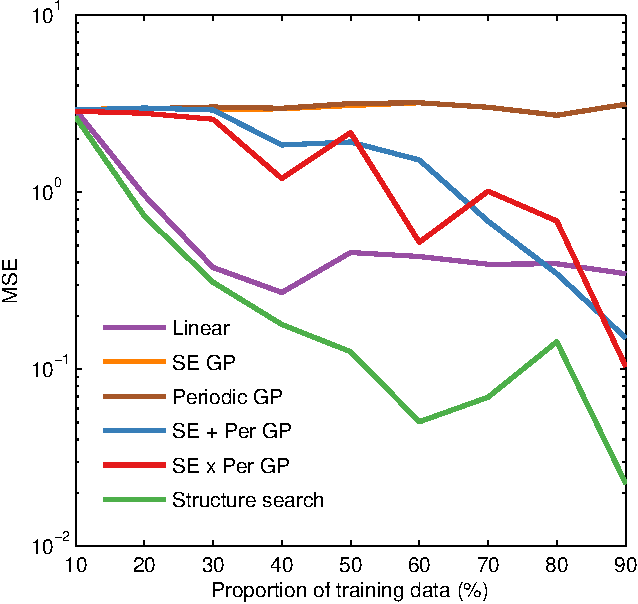
\includegraphics[width=0.95\columnwidth]{../figures/extrapolation_curves/01-airline-s-ex-curve_hint.pdf}
\end{tabular}
\caption{Extrapolation performance on the airline dataset.  Here, we show average test-set MSE as a function of the fraction of the dataset used for training. 
%\TBD{RBG: Are we using a fixed test set, or the complement of the training set?  It seems like we should do the former, so that the results are less noisy.}
}
\label{fig:extrapolation}
\end{figure}

\TBD{RBG: It's not clear what the procedure is. Are we doing the thing I suggested, where we hold out the last 0.1 and train on $0.9 - \alpha$ to 0.9?}

To test the extrapolation capabilities of our model against standard baselines, we computed predictive mean-squared-error as a function of the proportion of data used for training.
Figure \ref{fig:extrapolation} shows these learning curves, comparing against linear regression, and a variety of fixed kernel \gp{{} models.  

Linear regression models have fixed capacity, and quickly plateau in their predictive performance.  In contrast, a \gp{} with an SE or RQ kernel has unbounded capacity.  However, simply having unbounded capacity does not necessarily translate into the ability to extrapolate, as demonstrate in Figure \ref{fig:extrapolation}.  Only by increasing the amount of structure expressible in a model can we capture the regularities in the data that allow long-range extrapolation.

\TBD{Josh: Can you write about the Blessing of abstraction, and doing lots with a small amount of data?  This might become apparent from plotting the extraplolations.} \TBD{RBG: We could make this point as part of the learning curves for extrapolation by marking the points at which each additional aspect of the structure is found.}


\subsection{Interpolation}

\TBD{RBG: Zoubin made the comment that in high dimensions, all prediction is extrapolation. Would it be better to title this section something like ``high-dimensional prediction?''}

To demonstrate the interpolation accuracy of our method, we extended the comparison of \cite{duvenaud2011additive11} to include our method.
We compared 5 methods on 5 datasets in terms of mean-squared (MSE) error and predictive likelihood, averaging across 10 data folds.
Results are presented in tables \ref{tbl:Regression Mean Squared Error} and \ref{tbl:Regression Negative Log Likelihood}.  All bolded results are not significantly different from the best-performing method in each experiment in a paired t-test.
%
% --- Automatically generated by resultsToLatex2.m ---
% Exported at 28-Jan-2013 15:53:45
\begin{table*}[ht!]
\caption{{\small
Regression Mean Squared Error
}}
\label{tbl:Regression Mean Squared Error}
\begin{center}
\begin{tabular}{l | r r r r r}
Method & \rotatebox{0}{ bach  }  & \rotatebox{0}{ concrete  }  & \rotatebox{0}{ puma }  & \rotatebox{0}{ servo }  & \rotatebox{0}{ housing }  \\ \hline
Linear Regression & $1.031$ & $0.404$ & $0.641$ & $0.523$ & $0.289$ \\
GP GAM & $1.259$ & $0.149$ & $0.598$ & $0.281$ & $0.161$ \\
HKL & $\mathbf{0.199}$ & $0.147$ & $0.346$ & $0.199$ & $0.151$ \\
GP Squared-exp & $\mathbf{0.045}$ & $0.157$ & $0.317$ & $0.126$ & $\mathbf{0.092}$ \\
GP Additive & $\mathbf{0.045}$ & $\mathbf{0.089}$ & $\mathbf{0.316}$ & $\mathbf{0.110}$ & $0.102$ \\
%22-Jan & $\mathbf{0.513}$ & $\mathbf{0.089}$ & $\mathbf{0.312}$ & $\mathbf{0.095}$ & $\mathbf{0.091}$ \\
\hline
Structure Search & $\mathbf{0.044}$ & $\mathbf{0.087}$ & $\mathbf{0.315}$ & $\mathbf{0.102}$ & $\mathbf{0.082}$
\end{tabular}
\end{center}
\end{table*}
% End automatically generated LaTeX

% --- Automatically generated by resultsToLatex2.m ---
% Exported at 28-Jan-2013 15:53:45
\begin{table}[h!]
\caption{{\small
Regression Negative Log Likelihood
}}
\label{tbl:Regression Negative Log Likelihood}
\begin{center}
\begin{tabular}{l | r r r r r}
Method & \rotatebox{0}{ bach  }  & \rotatebox{0}{ concrete  }  & \rotatebox{0}{ puma }  & \rotatebox{0}{ servo }  & \rotatebox{0}{ housing }  \\ \hline
Linear Regression & $2.430$ & $1.403$ & $1.881$ & $1.678$ & $1.052$ \\
GP GAM & $1.708$ & $0.467$ & $1.195$ & $0.800$ & $0.457$ \\
GP Squared-exp & $\mathbf{-0.131}$ & $0.398$ & $0.843$ & $0.429$ & $0.207$ \\
GP Additive & $\mathbf{-0.131}$ & $\mathbf{0.114}$ & $\mathbf{0.841}$ & $\mathbf{0.309}$ & $0.194$ \\
22-Jan & $\mathbf{0.346}$ & $\mathbf{0.134}$ & $\mathbf{0.835}$ & $\mathbf{0.241}$ & $\mathbf{0.138}$ \\
28-Jan & $\mathbf{-0.141}$ & $\mathbf{0.065}$ & $\mathbf{0.840}$ & $\mathbf{0.265}$ & $\mathbf{0.059}$ \\
\end{tabular}
\end{center}
\end{table}
% End automatically generated LaTeX

%
Our method outperforms the other methods in all tests. \fTBD{Is it worth including the learned structures in the table?}
\TBD{RBG: Can we provide any information about the datasets, e.g. number of data points and number of dimensions?}

\paragraph{Details of methods}

Linear regression was included as a baseline, with noise variance set to the empirical variance on the training residuals.
%
Generalized Additive Models (GP GAM) were implemented through a \gp{} whose kernel is a sum of SE kernels across dimensions.
This model was included to demonstrate that the gain in predictive performance was not simply due to the inclusion of additive structure.
%
Additive \gp{} was run using SE as a base kernel, with at most ten degrees of interaction.
%
Hierarchical Kernel Learning (HKL)
%\footnote{Code for HKL available at \texttt{http://www.di.ens.fr/\textasciitilde fbach/hkl/}} 
was run using the all-subsets kernel, which corresponds to the same set of kernels as considered by the additive \gp{} with a squared-exp base kernel.  Because HKL does not produce a probabilistic prediction, it could not be included in Table \ref{tbl:Regression Negative Log Likelihood}.
%

\paragraph{Source code}All of the experiments in this paper were performed using the standard GPML toolbox\footnote{Available at \texttt{www.gaussianprocess.org/gpml/code/}}; code to perform all experiments is available on github.



%$k = 1$, $D = 8$, kernels are SE and RQ (\TBD{currently running other experiments that may be more canonical}).
%We have extended the comparison of \cite{duvenaud2011additive11} to include our method.

%Some points for discussion
%\begin{itemize}
%\item Experiments just using SE kernel can outperform additive kernel surprisingly. This is presumably a regularisation effect of using a finite depth search and/or BIC. We could make this a more Bayesian result (i.e.~more a property of the model) by placing a prior on kernels that depends on the number of components.
%\item Need to discuss design choices e.g.~$k$, depth of search, base kernels.
%\end{itemize}




\section{Discussion}

\begin{quotation}
``It would be very nice to have a formal apparatus that gives us some ‘optimal’ way of recognizing unusual phenomena and inventing new classes of hypotheses that are most likely to contain the true one; but this remains an art for the creative human mind.''
% In trying to practice this art, the Bayesian has the advantage because his formal apparatus already developed gives him a clearer picture of what to expect, and therefore a sharper perception for recognizing the unexpected.

\hspace*{\fill}\citet{Jaynes85highlyinformative}

%\emph{ E.T. Jaynes  from the last paragraph (p. 351) of his 1985 paper, “Highly Informative Priors.”}

\end{quotation}

%There has developed a large and mature literature on automatic structure discovery in unsupervised settings \fTBD{citations including Josh}.  
%For example, searches over large model classes have been succesfully used in machine vision \cite{pinto2009high}, analogous to high-throughput methods used in biology.
\TBD{RBG: I took out the prior work references since this doesn't seem like the right place to introduce them. If we want them, maybe move them to the related work section?  Also, note that the Pinto reference was supervised learning.}

%However, relatively little attention has been paid to automatic structure discovery in supervised learning. %\TBD{RBG: I don't think we need separate Discussion and Conclusion sections. I vote for getting rid of Discussion, since most of this is covered in the related work section anyway.}
%
%Our work respresents a step towards automated structure discover in supervised settings.
% data-based modeling, as opposed to proposing the model beforehand.

%In particular, this work removes the need for an expert to propose a kernel family in order to effectively use a Gaussian process model.  
%Choosing a kernel family is a stumbling block even for experts.
%Automating the search over kernel structures will make it easier for non-statisticians to construct appropriate models for their data.

The ability to learn kernel hyperparameters and combination weights automatically has been an important factor enabling the widespread use of kernel methods.
For the most part, however, it has been up to the user to choose the proper form for the kernel, a task which requires considerable expertise.

Towards the goal of automating this process, we introduced a space of composite kernels defined compositionally as sums and products of a small number of base kernels.
We proposed a search procedure for this space of kernels which parallels the process of scientific discovery.

We found that the learned structures are often capable of accurate extrapolation in complex time series datasets and are competitive with widely used kernel classes and kernel combination methods on a variety of prediction tasks.
The learned kernels often yield decompositions of a signal into diverse and interpretable components, which provides an additional degree of reassurance that the learned structure reflects the world.
We believe that a data-driven approach to choosing kernel structures automatically can help make nonparametric regression and classification methods accessible to non-experts.

%Machine learning can be more data-driven, analogous to the high-thoughput approaches being used in biology. 




%Indeed, the authors were sometimes surprised by the kernels chosen by the automated search, and the elegant ways in which complex structure was expressed through simple combination of kernels.



%\paragraph{Conclusion}

%In this paper, we introduced an automated search over composite kernels, defining the search space through a simple grammar consisting of a set of one-dimensional base kernels and operations which combine those kernels.

%We demonstrated that the composite structure search recovered interpretable\fTBD{Change to 'known' if we add those experiments} structure, and resulted in state-of-the-art predictive performance.  %We further demonstrated an automated decomposition of the posterior into a sum of interpretable components.

%\section{Future Work}

%\TBD{RBG: Do we need this section?  Bill hates future work sections since they basically just give the reviewers a list of things to complain about.}

%\paragraph{Support Vector Machines} Structure search could be used to select kernels for support vector machines, using cross-validated prediction error as an objective function.

%However, it would be presumably quite difficult to learn the moderate number of kernel hyperparameters present in composite kernels using only cross-validation.

%\paragraph{Noise Models and Mean Functions}
%The models used in this paper all assumed Gaussian noise, as well a constant mean function for the Gaussian process.
%A more sophisticated approach might also define grammars over composite mean functions and noise models.
%However, in most cases, the covariance function can express structure that might be expressed in the mean function, and often in a more flexible way.
%The same can be said about noise models - for instance, a t-noise can be approximated by a sum of sq-exp kernels with very small lengthscales, but output variances which vary widely.


%\paragraph{Bayes model averaging}
%A natural extension of this work is to average over models in the grammar with a Bayes model averaging approach.
%This would mean augmenting our grammar with a prior over kernel structures, and approximately integrating over both structures and kernels.  

%In the first few levels of the search, where the difference between likelihoods of different kernel structures is usually high, model averaging might not make a substantial difference in terms of prediction.
%However, at deeper levels of the kernel search, integrating over structures and parameters would address overfitting concerns.

%\paragraph{Parsimony}
%Integrating over kernel structures raises the problem of reporting interpretable structures to the user.
%Currently, this is achieved through the use of the BIC complexity penalty, and reporting only the highest-scoring structure found.
%In experiments which used the more sophisticated Laplace approximation as a complexity penalty, the kernels found were more complicated.

%\paragraph{Bayesian Optimization} 
%The greedy search strategy used in this paper is rudimentary.  A natural extension of this work would be a model-based search over composite kernels, where the results of previous searches are used to propose informative directions.  This would be an example of ``meta-learning''.
%\cite{snoek2012practical} [also cite Lizotte, de Frietas]
%
%\paragraph{A Kernel between kernels}
%Placing a \gp{} model on the log-likelihood of different kernels would require constructing a kernel on kernels, as in \cite{ong2002hyperkernels}.

\subsubsection*{Acknowledgements}

\bibliographystyle{format/icml2013}
\bibliography{gpss}
\end{document}



% Stuff that didn't make the cut

%Kernel-based nonparametric regression models have been widely and succesfully used over the last 20 years. [citations needed]
%As part of the development of this model class, a rich set of kernels have been developed for both continuous and structured data.
%Because different kernels reflect different properties of the function being modeled, the choice of kernel can have a large impact on the sorts of structure that can be expressed or discovered by the model.

%When approaching a new dataset, it is often not clear which kernel family is most appropriate, especially for non-experts.
%Often, a standard kernel family (typically squared-exponential) is chosen out of convenience, and kernel parameters are set by cross-validation or maximum marginal likelihood. [citations?]

%Sometimes the argument is made that since most kernels are universal (i.e. consistent in the limit), that the choice of kernel is not important[citation?].  However, our experiments demonstrate that for datasets of moderate size, predictive performance, extrapolation and interpretability all depend heavily on the choice of kernel. \TBD{RBG: Do people actually say the choice of kernel isn't important?  This sounds like a straw man...}

%\paragraph{Main contribution}
%In this paper, we introduce an automated search over composite kernels.
%We define the search space through a simple grammar consisting of a set of one-dimensional base kernels (squared-exp, periodic, linear, etc.) and operations which combine those kernels (add and multiply).
%Our objective function is the marginal likelihood of a Gaussian process model with the given kernel, conditioned on the data.

%We examine the composite kernels discovered by this search on several datasets, and demonstrate that they can recover known structure, and result in state-of-the-art predictive performance.  We further demonstrate that in some cases, the structured posterior can be automatically decomposed into a sum of interpretable components, e.g. in Figure \ref{fig:airline_decomp}. \TBD{RBG: Need to clarify that the contribution isn't that we can decompose it (that was in GPML), but that the decomposition is often interesting.}

%\section{Motivation}
%\TBD{RBG: Do we need a separate motivation section?  The introduction should motivate the work.}

%There is a large and mature literature on automatic structure discovery in unsupervised settings [citations including Josh].
%However, relatively little attention has been paid to automatic structure discovery in supervised learning.

%Similar searches over large model classes have been succesfully used in machine vision [cite Cox + Pinto].
%  This work respresents a step towards more data-based modeling, as opposed to proposing the model beforehand.
%In general, learning the model class from data seems superior proposing the model beforehand.
%In high dimensional problems, it is also hard for a practitioner to propose an appropriate model even after examining a dataset closely.
% Choosing a kernel family is also a stumbling block for non-experts who wish to use Gaussian Process models.

%Machine learning can be more data-driven, analogous to the high-thoughput approaches being used in biology. 

%\subsection{Convenience Priors}
%One of the main advantage of kernel methods, and Gaussian process regression in particular, is that the kernel can be used to specify interesting prior structure to the model.
%However, in practice, GPs are typically used with only the squared-exp kernel.
%[Apparently, this was one of Sholkopf's big dissapointment with GPs... is there a quote from him on this? -David]

%A frequent criticism of the Bayesian framework is that priors are often chosen purely for convenience. 
%Gaussian process priors may be a good examples of a model chosen for its tractability.
%However, specifying a compound kernel typically does not change the order of computational complexity of inference in Gaussian process models.
%The broad use of simple kernels may be simply due to the difficulty of determining which kinds of structure exist in the data.
%As well, even if one understands the structure present in a dataset, it is often non-obvious how to express that through a covariance function. 
%\TBD{RBG: Not sure we need this in the motivation. Is this basically just to answer the objection of why we don't consider the tradeoff between expressiveness and tractability?  Also, the prior can affect computational tractability if we're using approximate algorithms, so this makes it sound like we're only thinking about small datasets.}

%Automating the search over kernel structures should be especially useful in allowing pracitioners from a wide variety of backgrounds to use appropriate models for their data.
%Indeed, the authors were sometimes surprised by the kernels chosen by the automated search, and the elegant ways in which complex structure was expressed through simple combination of kernels.



\subsubsection{Data sets}

\paragraph{Bach Synthetic Dataset}
\fTBD{Too much text? Move to supplementary}
In addition to standard UCI repository datasets, we generated a synthetic dataset following the same recipe as \cite{DBLP:journals/corr/abs-0909-0844}.
% From a covariance matrix drawn from a Wishart distribution with 1024 degrees of freedom, we select 8 variables.
%We then construct the non-linear function $f(X) = \sum_{i=1}^4 \sum_{j=1+1}^4 X_i X_j + \epsilon$, which sums all 2-way products of the first 4 variables, and adds Gaussian noise $\epsilon$.
This dataset is one which can be predicted well by a kernel which is a sum of two-way interactions over the first 4 variables, ignoring the extra 4 noisy copies.
%
This dataset was designed by \cite{DBLP:journals/corr/abs-0909-0844} to demonstrate the advantages of HKL over a \gp{} with a SE-ARD kernel. 

%If the dataset is large enough, HKL can construct a hull around only those subsets of cross terms that are optimal for predicting the output.
%GP-ARD, in contrast, can only learn to ignore the noisy copy variables, but cannot learn to ignore the higher-term interactions between the predictive variables.
%However, a GP with an additive kernel can learn both to ignore irrelevant variables, and to ignore certain orders of interaction.
%In this example, the additive GP is able to recover the relevant structure.

[TODO: Describe concrete, pumadyn, servo and housing]


\subsection{Multidimensional decomposition}

\begin{figure*}[h!]
\centering
\begin{tabular}{ccc}
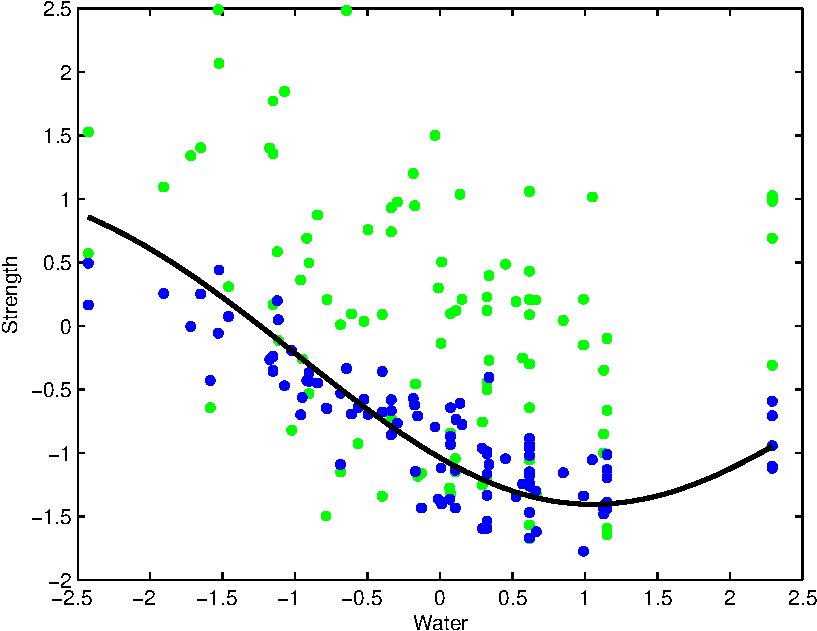
\includegraphics[width=0.3\textwidth]{../figures/additive_multi_d/interpretable_1st_order1.pdf} &
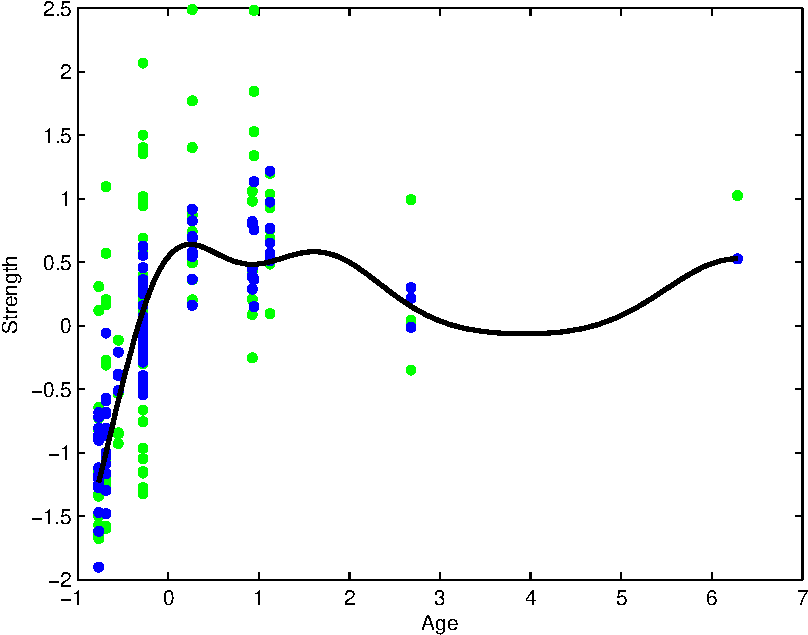
\includegraphics[width=0.3\textwidth]{../figures/additive_multi_d/interpretable_1st_order2.pdf}& 
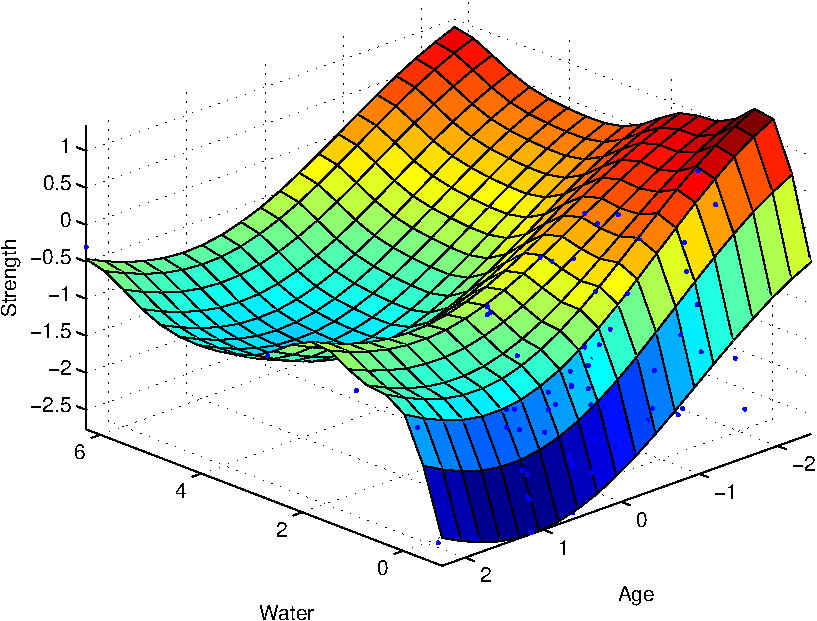
\includegraphics[width=0.3\textwidth]{../figures/additive_multi_d/interpretable_2nd_order1.pdf}\\
\end{tabular}
\caption{One-dimensional decompositions of the concrete dataset posterior.  Left, Centre:  Green points indicate the original data, blue points are data after the mean contribution from the other dimensions' first-order terms has been subtracted.  The black line is the posterior mean of a \gp{} with only one term in its kernel.  Right:  The posterior mean of a \gp{} with only one second-order term in its kernel.}
\label{fig:interpretable functions}
\end{figure*}
%
Figure \ref{fig:interpretable functions} demonstrates that an additive posterior can be decomposed into a sum of functions across dimensions.
